\section{Results}
\subsection{Model Selection}

\begin{frame}{Results of Model Selection}
    \begin{table}[ht]
\caption{F1 Score for Pathological findings classification task with Vindr, comparing different Deep Learning Models.}
\label{tab:f1score}
\centering
\resizebox{\textwidth}{!}{%
\begin{tabular}{@{}lS[table-format=2]SSSSSS@{}}
\toprule
                         & {N}    & {DenseNet} & {EfficientNet} & {ResNet50} & {SwinTransformer} & {VGG19}   & {MobileNet} \\ \midrule
Mass                     & 237 & 0.7828   & 0.81513      & 0.74163  & 0.76984         & 0.75584 & 0.70833   \\
Suspicious Calcification & 115 & 0.84746  & 0.86463      & 0.85973  & 0.82759         & 0.87288 & 0.82819   \\
Assymetries              & 79  & 0.30645  & 0.29508      & 0.2      & 0.31034         & 0.20370 & 0.32432   \\
Suspicious Lymph Node    & 11  & 0.66667  & 0.5          & 0.73684  & 0.37037         & 0.4     & 0.47619   \\ \midrule
Weighted Average        & 442 & 0.71159  & \bfseries 0.72721 & 0.67543  & 0.69280    & 0.67875 & 0.66511   \\ \bottomrule
\end{tabular}%
}%
\end{table}

    \emph{EfficientNet} has the best overall performance, with an F1 score of \num{0.727}. We chose this model as the backbone for our classifier.
\end{frame}

\subsection{Classifier}
\begin{frame}{Results of our Classifier}
    \begin{columns}
        \begin{column}{0.65\textwidth}
            \begin{table}[ht]
    \centering
    \caption{Metrics of pathological findings classification task using Vindr}
    \resizebox{0.95\textwidth}{!}{%
    \begin{tabular}{p{0.3\textwidth}SSSSS[table-format=4]}
        \toprule
        & {Accuracy} & {Precision} & {Recall} & {F1} & {Support} \\
        \midrule
        No Finding               & 0.9780 & 0.9909 & 0.9844 & 0.9876 & 3643 \\
        Mass                     & 0.9697 & 0.7425 & 0.7300 & \bfseries 0.7362 &  237 \\
        Suspicious Calcification & 0.9902 & 0.8049 & 0.8609 & \bfseries 0.8319 &  115 \\
        Focal Asymmetry          & 0.9834 & 0.2000 & 0.0943 & 0.1282 &   53 \\
        Architectural Distortion & 0.9929 & 0.2222 & 0.0833 & 0.1212 &   24 \\
        Asymmetry                & 0.9951 & 0.0000 & 0.0000 & 0.0000 &   20 \\
        Suspicious Lymph Node    & 0.9978 & 0.6250 & 0.4545 & 0.5263 &   11 \\
        Skin Thickening          & 0.9980 & 1.0000 & 0.3333 & 0.5000 &   12 \\
        Nipple Retraction        & 0.9980 & 0.0000 & 0.0000 & 0.0000 &    7 \\
        Global Asymmetry         & 0.9983 & 0.0000 & 0.0000 & 0.0000 &    6 \\
        Skin Retraction          & 0.9993 & 0.5000 & 0.3333 & 0.4000 &    3 \\
    \bottomrule
    \end{tabular}
    }%
    \label{tab:best_model}
\end{table}
        \end{column}
        \begin{column}{0.35\textwidth}
            Our model achieves a weighted Accuracy of \SI{93.80}{\percent} and a weighted F1 score of \num{0.9557}
        \end{column}
    \end{columns}
    
\end{frame}

\subsection{Sliding patches}
\begin{frame}{Prediction on local windows}
    \begin{figure}
        \centering
        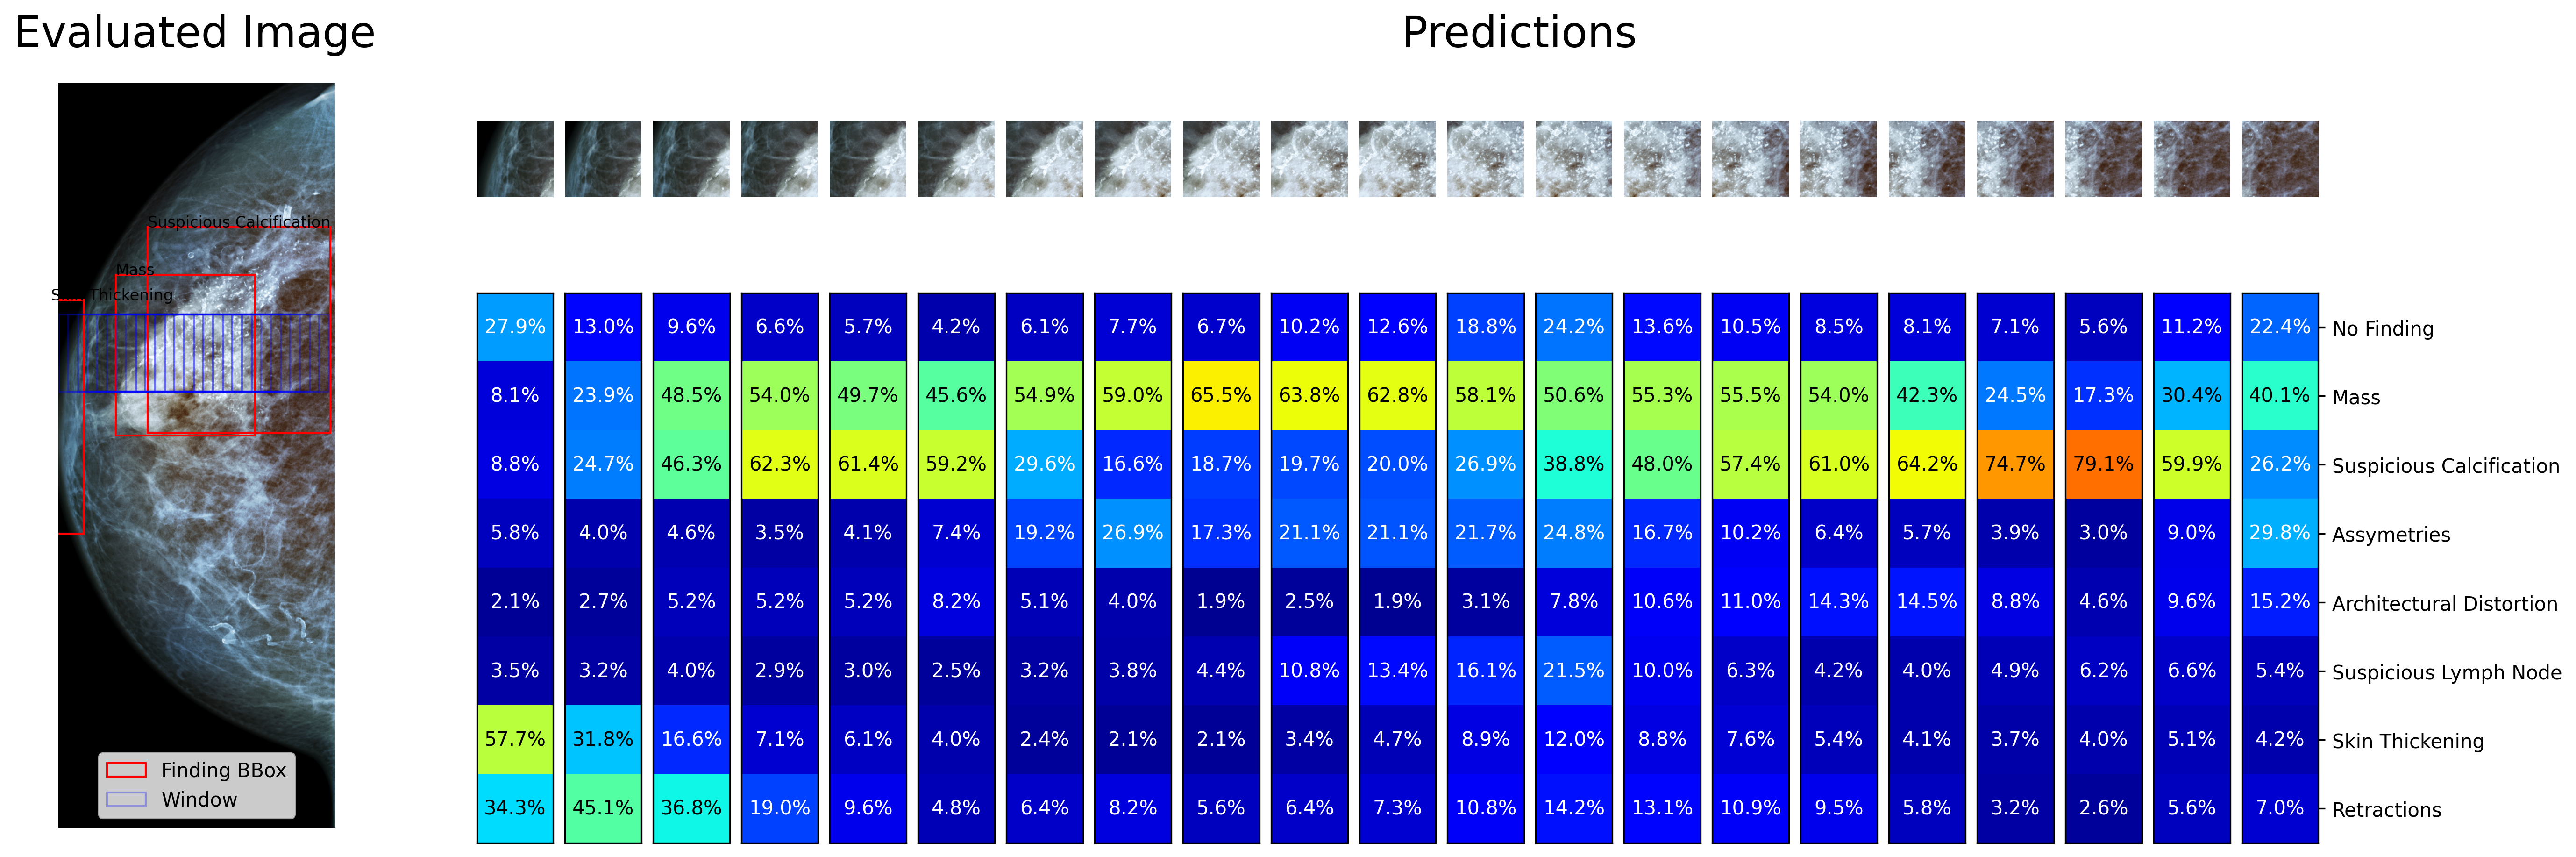
\includegraphics[width=\textwidth]{imagenes/pred_ventanas.png}
        \caption{Image with bounding boxes of its findings and prediction of a row of local windows using our classifier.}
    \end{figure}
\end{frame}

\begin{frame}{Heatmap}
    \begin{figure}
        \centering
        \includegraphics[width=\textwidth]{imagenes/prediction.png}
        \caption{Cropped test image with bounding boxes of its findings, feature activation heatmap, and prediction of the classifier.}
    \end{figure}
\end{frame}

\subsection{Scales}
\begin{frame}{Effects of scale of window}
    \begin{figure}
        \centering
        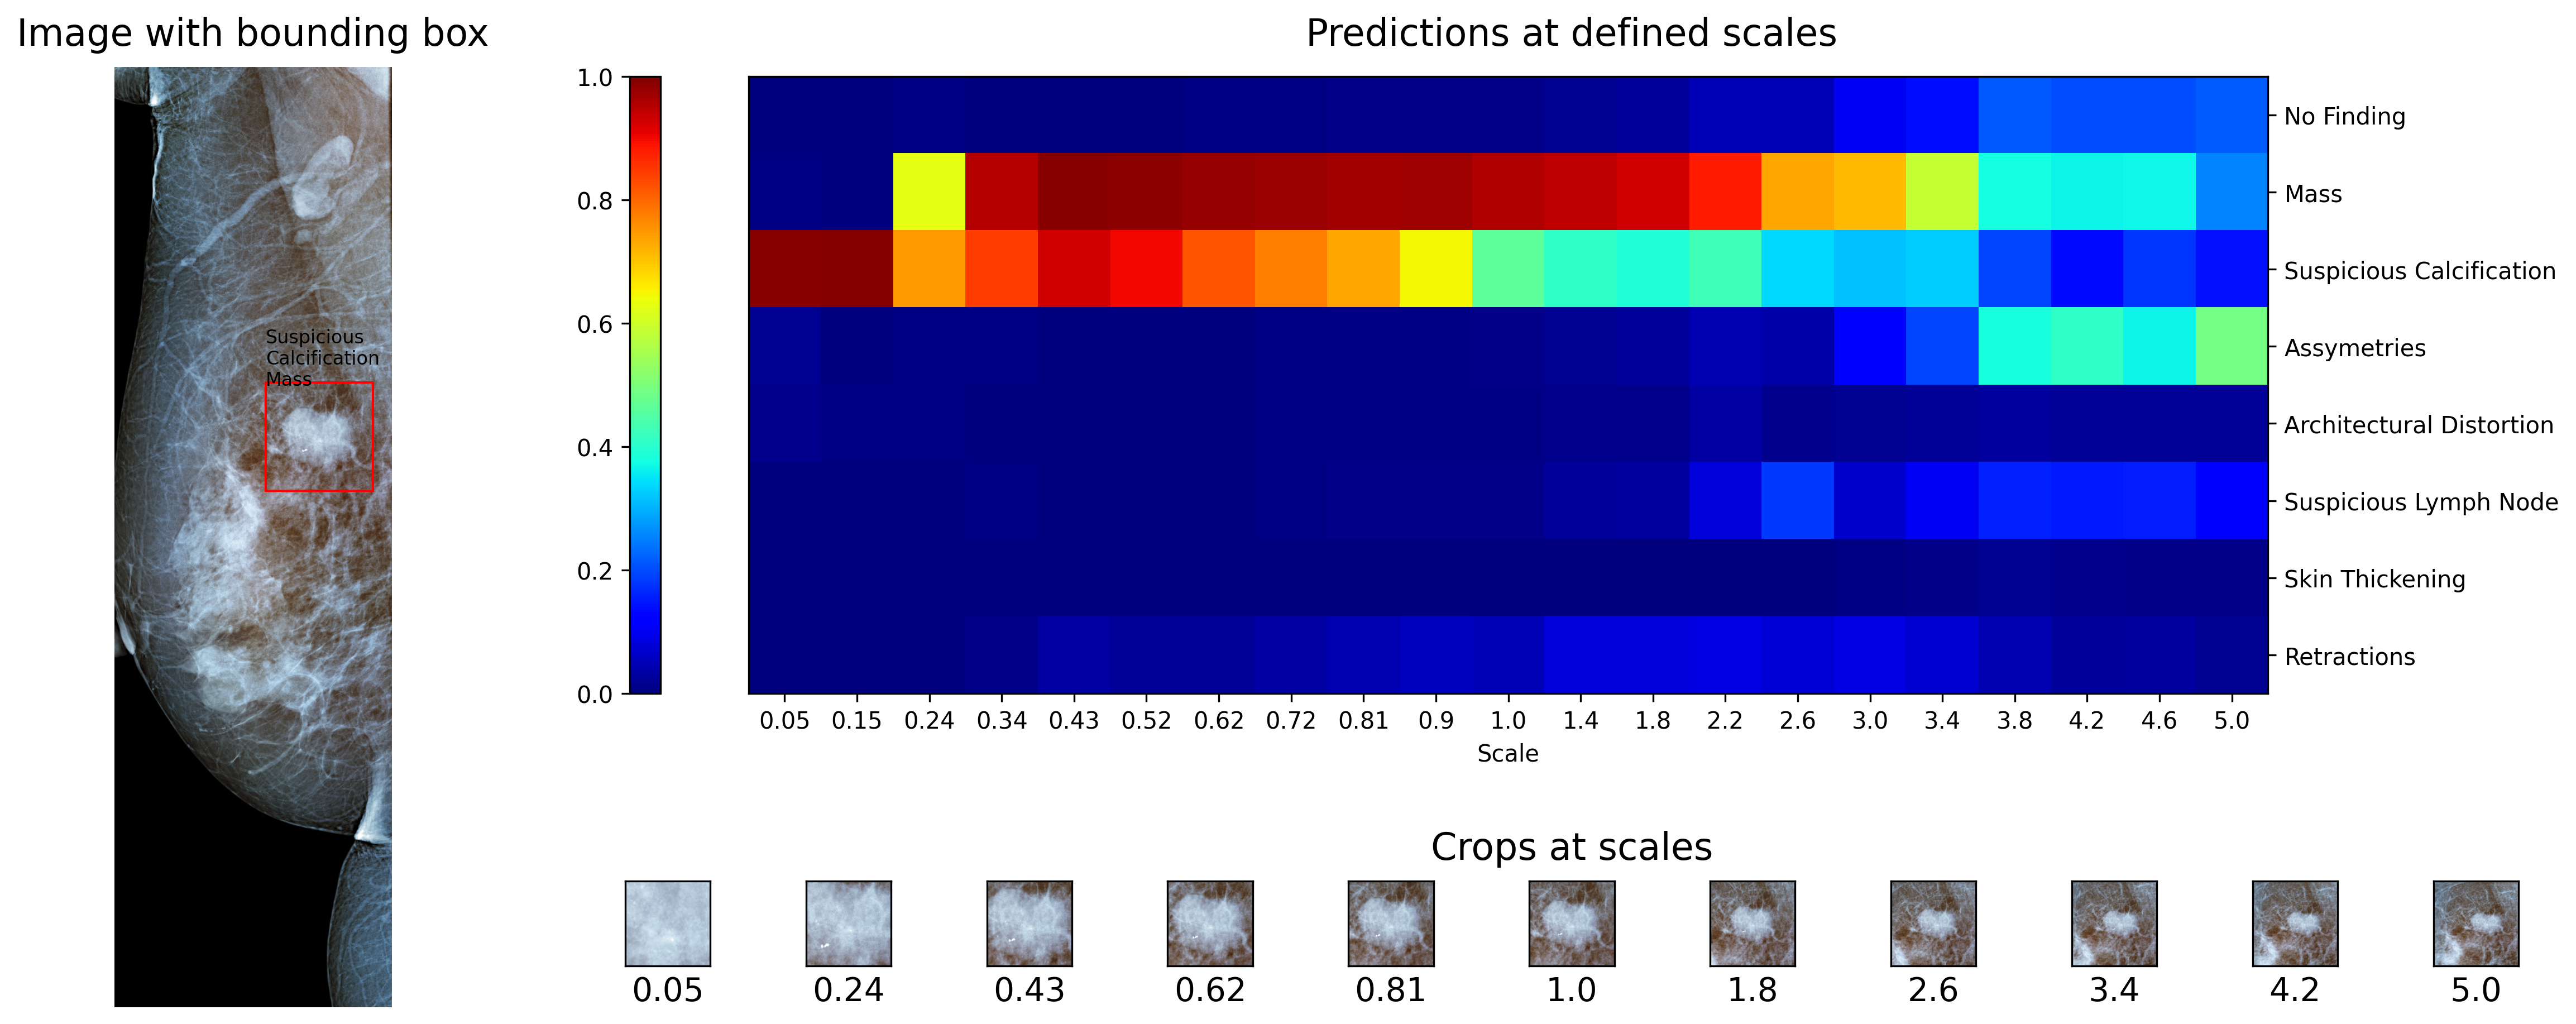
\includegraphics[height=0.7\textheight,keepaspectratio]{imagenes/ratios.png}
        \caption{Prediction of classifier, using finding at different scales.}
    \end{figure}
    
\end{frame}